\subsection{Stable Marriage Problem}
The \textit{stable marriage problem} is concerned with assigning pairings of partners between two distinct sets $A$ and $B$. The assignment of pairs is said to be a \textit{stable marriage} if there exists no elements $a \in A$ and $b \in B$ such that $a$ and $b$ are not paired together yet would prefer each other over their current partners \citep{McVitie1971}. This concept is demonstrated in Figure \ref{fig:smp}. The \textit{Gale and Shapely algorithm} can be used to find a stable marriage between the sets $A$ and $B$, provided that they are disjoint \citep{McVitie1971}. 

\begin{figure}[t]
    \centering
    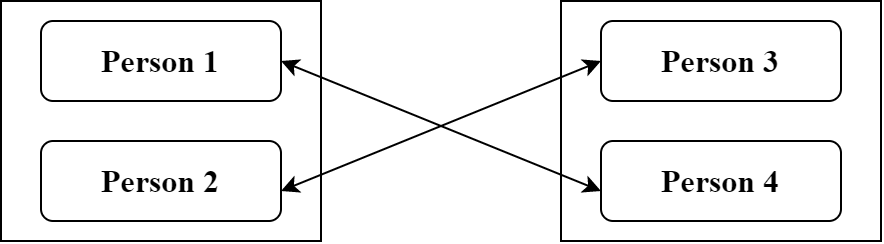
\includegraphics[height = .125\textheight]{stablemarriageproblem.png}
    \caption{An example of expressed preferences between two disjoint sets. In this case, Person $1$ and Person $4$ prefer each other and Person $2$ and Person $3$ prefer each other. Pairing Person $1$ with Person $4$ and Person $2$ with Person $3$ results in a stable marriage. Any other assignment would result in an unstable marriage.}
    \label{fig:smp}
\end{figure}

Consider a generic online dating service and assume that the collection of this service's users, its \textit{user base}, can be divided into two disjoint sets $A$ and $B$. These users will cease further use of the service if assigned into a stable marriage as they will be unable to find a partner they consider better. Assuming the rate at which the user base grows through new users is lower than the rate at which users leave the service, the service will soon go out of business.

Realistically, the conditions for the Gale and Shapely algorithm are not met in Tinder. Foremost, the two sets of partners must be disjoint \citep{McVitie1971} to guarantee the existence of a stable marriage. Traditionally these sets are assumed to be composed of heterosexual men and women respectively, but this is not the case for Tinder where gender preference can be set regardless of the user's own gender \citep{Courtois2018}. That is to say, if Tinder's user base were divided into two sets, there is no guarantee that a member of one set would not prefer another member of the same set. Additionally, the stable marriage problem typically requires that members of one set rank the members of the other set in order of preference and vice versa \citep{McVitie1971}. Tinder does not allow ranking, instead opting for a simple approve/disapprove system. These shortcomings require the stable marriage problem to be applied within the context of graph theory.